\chapter{The Scope of Research}
This chapter outlines the aim of the research within its objectives and boundaries. The following sections define the boundaries of Cloud Manufacturing systems and explain the scope of research to identify the Author’s perspective on applying distributed Cloud Manufacturing systems within an autonomous resources scenario.\\
\section{Research Motivation and Gaps}
This work is motivated by the need for practicable and applicable Cloud Manufacturing systems that can be temporary and dynamically created ad hoc to satisfy specific market demand in a sustainable way.\\
The transformation of existing manufacturing systems to new advanced and complex systems, such as Cloud Manufacturing, can be seen as a big challenge for any enterprise. This transformation poses new uncertainties in the new system that can impact every aspect of the operations lifecycle from design and engineering to the implementation final operations of the new manufacturing model. So, there is a need to understand and tackle uncertainties in cloud manufacturing networks derived from the introduction of resource autonomy and resource independence from a specific platform. To address these issues, steps needed to be followed, including understand and define key factors, main actors, and dynamics inside such networks; identify main issues that arise from the trade-off between decentralized governance and the need for centralized control in global scheduling, load balance and logistics optimization to provide long-term sustainability of the network; and develop a framework to implement such networks in a Cloud Manufacturing environment.\\
\section{Aims and objectives of the research}
The research aim is to develop a framework to manage operations in cloud manufacturing for autonomous resources. The framework comprises a taxonomy of the proposed architecture; a Multi-Agent System model to tackle coordination and communication issues; a detailed list of platform services, agents, and functionalities; a unique algorithm to determine local optimization in a job order combining logistics and distributed multi-task scheduling optimization; and the implementation process of a prototype with basic functionalities of the Multi-Agent System model.\\
Previous research has shown that most Cloud Manufacturing architectures require central governance and high investment for increasing efficiencies and capabilities across the product life cycle. This research aims to investigate the possibility for a Cloud Manufacturing platform constituted by independent and autonomous service providers and a set of clear founding principles to be deployable and viable for a homogenous manufacturing scenario.\\
The following objectives have been identified to track the progress of the research and ensure that the aim is achieved:
\begin{enumerate}
    \item Identification and analysis of existing research gaps in the context of Cloud Manufacturing Architectures.
    \item Development of a framework for a sustainable Cloud Manufacturing platform constituted by autonomous service providers
    \item Realization of implementation models for critical areas inside the framework
    \item Validation of the proposed models
\end{enumerate}
\section{Research Methodology}
The following steps, as shown in Figure \ref{fig:research-steps}, will be undertaken to verify the validity of the proposed framework and achieve the research aim:
\begin{enumerate}
    \item Review of the relevant literature on industry 4.0, cloud computing, cloud manufacturing, and smart manufacturing
    \begin{enumerate}
        \item Studies of Cloud Manufacturing: The state-of-the-art of Cloud Manufacturing will be reviewed to identify and demonstrate its impact.
        \item Review of cloud manufacturing frameworks regarding governance, architecture layouts, scheduling methods, virtualization of manufacturing resources and capabilities.
    \end{enumerate}
    \item Selecting a cloud manufacturing approach
    \begin{enumerate}
        \item In this section, a review of cloud manufacturing frameworks will be conducted, and the results are analyzed based on functional requirements, business constraints, and technology constraints to adopt a suitable approach for system deployment.
    \end{enumerate}
    \item Designing of a Cloud Manufacturing framework
    \begin{enumerate}
        \item Based on research gaps identified in the previous steps and the
outcomes of the last research step, a theoretical framework will be formulated to address cloud manufacturing system requirements. Additionally, a Cloud Manufacturing network will be implemented to form the baseline for analyzing the optimization problem and identifying critical parameters for a deploying approach.
    \end{enumerate}
    \item Implementation and validation of the proposed architecture
    \begin{enumerate}
        \item Development of implementation models of the proposed architecture focusing on specific critical areas.
        \item Validation through Multi Agents System simulation and numerical examples of the analytical optimization model.
    \end{enumerate}
\end{enumerate}

\begin{figure}[h]
    \centering
    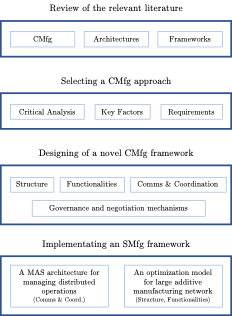
\includegraphics[height=10cm,keepaspectratio]{images/research-steps}
    \caption{Research Steps}
    \label{fig:research-steps}
\end{figure}
